\documentclass[11pt,a4paper]{article}
\usepackage[utf8]{inputenc}
\usepackage[english]{babel}
\usepackage{amsmath}
\usepackage{bbm}
\usepackage{amsthm}
\usepackage{amsfonts}
\usepackage{amssymb}
\usepackage{graphicx}
\usepackage{lmodern}
\usepackage{stmaryrd}
\usepackage{url}
\usepackage[left=2cm,right=2cm,top=2cm,bottom=2cm]{geometry}
\title{Convolution rapide par des noyaux radiaux}
\author{Martin}
\begin{document}
\renewcommand{\proofname}{Preuve}
\maketitle
\theoremstyle{plain}
\newtheorem{The}{Théorème}[section]
\newtheorem{Prop}{Proposition}[section]
\newtheorem{Cor}{Corollaire}[section]
\newtheorem{Lem}{Lemme}[section]
\theoremstyle{definition}
\newtheorem{Def}{Définition}[section]
\newtheorem{Rem}{Remarque}[section]
\newcommand{\enstq}[2]{\left\{#1\mathrel{}\middle|\mathrel{}#2\right\}}
\newcommand{\Lp}[2]{L^#1(#2)}
\newcommand{\Sob}[3]{W^{#1,#2}(#3)}
\newcommand{\RN}[0]{\mathbb{R}^N}
\newcommand{\norm}[1]{\left\|#1\right\|}
\newcommand{\sinc}[0]{\textup{sinc}}
\newcommand{\functionDef}[5]{\begin{array}{lllll}
#1 & : & #2 & \longrightarrow & #3 \\
 & & #4 & \longmapsto &\displaystyle #5 \\
\end{array}}
\newcommand{\N}{\mathbb{N}}
\newcommand{\D}{\mathbb{D}}
\newcommand{\A}{\mathcal{A}_{a,b}}
\newcommand{\Crad}{C^\infty_{rad}(\D)}
\newcommand{\Lrad}{L^2_{rad}(\D)}
\newcommand{\Lradab}{L^2_{rad}(\mathcal{A}_{a,b})}
\newcommand{\duality}[2]{\left\langle #1,#2\right\rangle}
\newcommand{\Hrad}{H^1_{rad}(\D)}
\newcommand{\Hzrad}{H^1_{0,rad}(\D)}

\section{Vecteurs propres du Laplacien sur la boule unité}

On étudie dans cette section les vecteurs propres radiaux du Laplacien avec conditions de Dirichlet sur le disque unité de $\mathbb{R}^N$, noté $\D$. 


\subsection{Distributions radiales}


\begin{Def} Pour tout $\varphi\in \mathcal{D}(\mathbb{R}^N)$ et pour toute matrice $A \in \mathcal{M}_N(\mathbb{R})$ on note $\sigma_A\varphi$ la fonction de $\mathcal{D}(\mathbb{R}^N)$ définie par \[\sigma_A\varphi(x) = \varphi(Ax)\]
\end{Def}
\begin{Def} On dit qu'une distribution $T$ est radiale si pour toute fonction test $\varphi$ et pour toute rotation $R \in O_N(\mathbb{R})$ on a \[\langle
T,\sigma_R\varphi\rangle\ = \langle T, \varphi\rangle\]  
\end{Def}
\begin{Prop} Pour toute fonction $\varphi \in \mathcal{S}(\mathbb{R^N})$, et pour toute matrice A inversible, si l'on note $\sigma_A\varphi(x) = \varphi(Ax)$, on a \[\mathcal{F}(\sigma_A\varphi) = \left|\dfrac{1}{\det(A)}\right|\left(A^{-1}\right)^T\mathcal{F}(\varphi)\] Où $\mathcal{F} $ désigne la transformation de Fourier. 
\end{Prop}
\begin{Cor} La transformée de Fourier commute avec les rotations. 
\end{Cor}


\begin{Prop} La transformée de Fourier d'une distribution tempérée radiale est une distribution radiale. 
\end{Prop}
\begin{proof} Soit $T$ une distribution radiale tempérée, $R$ une rotation et $\varphi \in \mathcal{S}(\mathbb{R}^N)$, alors

\[\begin{array}{ll}
\duality{\hat{T}}{\sigma_R\varphi} &= \quad\duality{T}{\widehat{\sigma_R\varphi}}\\
 &= \quad\duality{T}{\sigma_R\hat{\varphi}}\\
 &= \quad\duality{T}{\hat{\varphi}}\\
 &= \quad\duality{\hat{T}}{\varphi}
\end{array}\]


\end{proof}

Nous avons besoin de la définition de l'intégrale sur la surface de l'hypersphère, empruntée à \cite[p.78]{MR1681462} : 
\begin{Prop} Il existe une (unique) mesure de Borel $\sigma$ sur l'ensemble $\mathbbm{S}^{N-1} = \enstq{x  \in \mathbb{R^N}}{|x| = 1}$  telle que pour toute fonction intégrable $f$ sur $\mathbb{R^N}$ \[\int_{\mathbb{R^N}}f(x)dx = \int_{0}^{+\infty} \int_{\mathbbm{S}^{N-1}}r^{N-1}f(ru)d\sigma(u)\]
De plus, on a \[\sigma(\mathbbm{S}^{N-1}) = \frac{2\pi^{N/2}}{\Gamma(N/2)}\]
On note $c_N = \sigma(\mathbbm{S}^{N-1})$
\end{Prop}

\begin{Prop} Pour toute fonction $\varphi$ de classe $\mathcal{C}^\infty$ sur $\mathbb{R}^N$, la fonction $\textup{Rad}{\varphi}$ définie par \[ \textup{Rad}{\varphi}(x) = \frac{1}{c_N}\int_{S^{n-1}}\varphi(|x|u)d\sigma(u)\]
est de classe $\mathcal{C}^\infty$ sur $\mathbb{R}^N$. 

\begin{proof}
La régularité en dehors de l'origine est évidente. 
Il est plus facile de montrer la régularité en $0$ de $\textup{Rad}{\varphi}(x)$ en utilisant l'expression équivalente \[\textup{Rad}{\varphi}(x) = \int_{R\in O_N(\mathbb{R})} \varphi(Rx) d\mu_h (R)\]
où $\mu_h$ désigne la mesure de Haar normalisée sur le groupe $O_N(\mathbb{R})$. L'équivalence entre les deux expressions est traitée dans le premier chapitre de \cite{milman2009asymptotic}. On peut alors exprimer la différentielle n-ième de $\textup{Rad}{\varphi}(x)$ en fonction de celle de $\varphi$ comme suit : \[D^n\textup{Rad}{\varphi}(x)[h_1,...,h_n] = \int_{R\in O_N(\mathbb{R})} D^n\varphi(Rx)[Rh_1,...,Rh_n]d\mu_h(R)\]
On voit alors que $\textup{Rad}{\varphi}(x)$ est dérivable à tout ordre en $0$.
\end{proof}

\end{Prop}

\begin{Def} On définit l'application $\textup{Rad}$ par \[\functionDef{\textup{Rad}}{\mathcal{C}^\infty(\mathbb{R}^N)}{\mathcal{C}^\infty(\mathbb{R}^N)}{\varphi}{x\longmapsto\frac{1}{c_N}\int_{S^{n-1}}\varphi(|x|u)d\sigma(u)}\]
\end{Def}

\begin{Prop} L'application Rad stabilise $\mathcal{D}(\mathbb{R}^N)$ et $\mathcal{S}(\mathbb{R}^N)$
\begin{proof}
Il est évident que si $\varphi$ est à support compact, $\textup{Rad}\varphi$ l'est aussi. Pour le second point, il suffit de montrer que lorsque $\varphi$ est à décroissance rapide, $\textup{Rad}\varphi$ l'est aussi. Exprimons les dérivées partielles de $\textup{Rad}\varphi$. Notons $(f_1,f_2,...,f_N)$ la base canonique de $ \mathbb{R}^N$, on a alors pour tout multi-indice $\alpha$  \[\partial^\alpha \varphi(x) = D^{|\alpha|}\varphi(x)[\underbrace{f_1,...,f_1}_{\alpha_1 \textup{ fois}},\underbrace{f_2,...,f_2}_{\alpha_2 \textup{ fois}},...,\underbrace{f_N,...,f_N}_{\alpha_N \textup{ fois}}] \] Pour tout multi-indice $\alpha$ et toute matrice $A$ contenant en colonne les vecteurs $a_1$, ..., $a_N$, nous notons par la suite $C(A,\alpha) = (\underbrace{a_1,...,a_1}_{\alpha_1 \textup{ fois}},...,\underbrace{a_N,...,a_N}_{\alpha_N \textup{ fois}})$. Soient $\alpha$ et $\beta$ deux multi-indices, on peut écrire \[ x^\alpha \partial^\beta \textup{Rad}\varphi(x) = \int_{R\in O_N(\mathbb{R})} x^\alpha D^{|\beta|}\varphi(Rx)[C(R,\beta)]dR\] D'où \[ \left|x^\alpha \partial^\beta\textup{Rad}\varphi(x)\right| \leq \int_{R\in O_N(\mathbb{R})} \left\|Rx\right\|^{|\alpha|} \left\|D^{|\beta|}\varphi(Rx)\right\|dR\]
Car $\|x\| = \left\|Rx\right\|$ (les rotations sont des isométries) et donc on voit que le membre de droite tend vers 0 lorsque $\|x\| \to + \infty$ (par le théorème de convergence dominée), donc $\textup{Rad}\varphi$ est à décroissance rapide. 
\end{proof} 
\end{Prop}

\begin{Prop} Pour toute distribution radiale $T$ et toute fonction test $\varphi$, on a \[\duality{T}{\varphi} = \duality{T}{\textup{Rad}\varphi}\]
\begin{proof}
L'intégrale commute avec le crochet de dualité. 
\end{proof}
\end{Prop}


\subsection{Espaces de fonctions radiales}


\begin{Def} On définit l'espace $\Lrad = \enstq{f\in L^2(\D)}{\exists g \in L^1_{loc}(\D) : f(x) = g(|x|) \text{ p.p. }}$, que l'on munit du produit scalaire usuel sur $L^2(\D)$. C'est un espace de Hilbert, comme sous-espace fermé de l'espace $L^2(\D)$. 	
\end{Def}

\begin{Def} On note $\Crad$ l'espace des fonctions infiniment dérivables, à support compact et radiales : \[C^\infty_{rad}(\D) = \enstq{f\in C^\infty_c(\D)}{|x| = |y| \implies f(x) = f(y)}\]
\end{Def}


\begin{Prop}
L'espace des fonctions $\Crad$ est dense dans $\Lrad$  
\begin{proof}
On sait que l'espace $C^\infty_c(\D)$ est dense dans $L^2(\D)$. Soit $f \in \Lrad$ et $\varepsilon > 0$, montrons qu'on peut trouver une fonction $h$ de $\Crad$ telle que $\norm{f - h}_{L^2(\D)} < \varepsilon$. Nous savons qu'il existe $\chi \in C^\infty_c(\D)$ vérifiant cette relation. Posons $h = \textup{Rad}\chi \in \Crad$.
L'inégalité de Jensen appliquée à la mesure $\dfrac{\sigma}{c_N}$ permet alors d'assurer que $\norm{f - h}_{L^2(\D)} < \varepsilon$. 
\end{proof}
\end{Prop}

\begin{Def} On définit l'espace $\Hrad= \enstq{f\in \Lrad}{\forall i \in [1,N], \partial_i f  \in \Lrad}$ muni du produit scalaire \[(u,v) = \int_{\D} uv + \nabla u \nabla v\] C'est un sous-espace fermé de $H^1(\D)$ donc un espace de Hilbert. 
\end{Def}

\begin{Prop} L'injection canonique de $\Hrad$ dans $\Lrad$ est compacte. 
\begin{proof} C'est un corollaire du théorème de Rellich. En effet, si une suite de fonction radiales de $H^1(\D)$ est bornée, on peut en extraire une sous-suite convergente dans $L^2(\D)$  et on vérifie que la limite est nécessairement radiale. 
\end{proof}

\end{Prop}

\begin{Def} On définit l'espace $\Hzrad$ comme l'adhérence de $\Crad$ dans $H^1_{rad}$. On remarque que $\Hzrad$ est dense dans $\Lrad$ puisque $\Crad$ est dense dans ces deux espaces.  
\end{Def}

\begin{Prop} La norme $\Hrad$ est équivalente à la norme \[\norm{u}_{\Hzrad} = \int_\D |\nabla u|^2\]. 

\begin{proof}
C'est une conséquence classique de l'inégalité de Poincaré. 
\end{proof}
\end{Prop}




\subsection{Base de vecteurs propres radiaux du Laplacien avec conditions de Dirichlet}

\begin{The} Il existe une base de $\Lrad$ formée de fonctions radiales de classe $C^\infty(\D)$ qui sont des vecteurs propres du Laplacien avec condition de Dirichlet sur la boule unité i.e. 
\[\exists (e_n)_{n\in \mathbb{N}} \in C^\infty(\D), \quad (\lambda_n)_{n\in \mathbb{N}} \in \mathbb{R}^+ : \quad \Delta e_n = - \lambda_n e_n\] avec $|x| = 1 \implies e_n(x) = 0$ 
où $(e_n)_{n\in\mathbb{N}}$ est une base hilbertienne de $\Lrad$. La suite des valeurs propres $\lambda_n$ tend vers $+\infty$. 
\begin{proof}
Nous avons vérifié dans la sous-section précédente toutes les hypothèses nécessaires pour appliquer le théorème 7.3.2 de \cite[p. 219]{allaire2005analyse}. Nous en déduisons l'existence d'une base Hilbertienne de $\Lrad$ formée des vecteurs propres du Laplacien sur $\Hzrad$ et la suite des valeurs propres positives tend vers l'infini. La régularité des vecteurs propres provient du théorème de régularité elliptique. 
\end{proof}
\end{The}

\begin{Prop} Notons $g_n$ les fonctions définies sur $[0,1]$ par $g_n(r) = e_n(rw)$ où $w$ est un vecteur quelconque de norme $1$. Les fonctions $g_n$ sont de classe $\mathcal{C}^{\infty}$ sur $[0,1]$ et sont solutions sur $]0,1[$ de l'équation différentielle du second ordre : 
\begin{equation}g_n''(r) + \frac{N-1}{r} g_n'(r) + \lambda_n g_n(r) = 0    
\label{eqDiffVecPropre}
\end{equation}
\begin{proof}
Cela vient de l'expression classique du Laplacien en coordonnées sphériques. 
\end{proof}
\end{Prop}

\begin{Prop} Toutes les valeurs propres $\lambda_n$ définies précédemment sont simples
\begin{proof}
Considérons deux vecteurs propres $e_1$ et $e_2$ du Laplacien dans l'espace $\Lrad$ associés à une même valeur propre $\lambda$, et $g_1$ et $g_2$ les fonctions définies sur $[0,1]$ par $g_i(r) = e_i(rw)$ où $w$ est un vecteur unitaire quelconque. Considérons $\tilde{g}_1$ et $\tilde{g}_2$ les solutions maximales de l'équation différentielle  (\ref{eqDiffVecPropre}) sur $I = \mathbb{R}_+^*$ avec conditions de Cauchy respectives \[\tilde{g}_1(1) = 0, \quad\tilde{g}_1'(1) = g_1'(1)\] \[\tilde{g}_2(1) = 0, \quad \tilde{g}_2'(1) = g_2'(1)\] En vertu du théorème de Cauchy-Lipschitz, $\tilde{g}_2'(1) \neq 0$ sinon on aurait $\tilde{g}_2 = 0$, impliquant $g_2 = 0$ et donc $e_2=0$. \\La fonction \[\tilde{g} = \dfrac{\tilde{g_1}'(1)}{\tilde{g_2}'(1)}\tilde{g}_2\] est bien définie et est une solution maximale du même problème de Cauchy que $\tilde{g}_1$. On en déduit que $\tilde{g} = \tilde{g_1}$ d'où $\tilde{g_1}$ et $\tilde{g_2}$ sont proportionnelles et donc $g_1$ et $g_2$ aussi. On a donc montré que $e_1$ et $e_2$ sont proportionnelles. 
\end{proof}
\end{Prop}

\begin{The} Les distributions tempérées radiales vérifiant  \begin{equation}
- \Delta f = f
\label{defJf}
\end{equation}
sont toutes proportionnelles à la fonction \begin{equation}
J(x) = \frac{1}{c_N}\int_{\mathbbm{S}^{N-1}} e^{ix \cdot u}d\sigma(u)
\label{defJFourier}
\end{equation} 
\begin{proof}
La preuve peut se faire de manière indirecte en montrant que l'expression proposée fournit bien une solution, et en utilisant les résultats bien connus sur les fonctions de Bessel pour l'unicité. Nous avons eu la "curiosité" de chercher une démonstation directe, ce qui rendait nécessaire la formalisation faite précédemment. Nous en donnons d'abord une présentation intuitive mais non rigoureuse avant de donner une preuve plus formelle. On peut réécrire l'équation  (\ref{defJf}) dans le domaine de Fourier : \begin{equation}
\left(|\xi|^2-1\right)\hat{f}(\xi) = 0
\end{equation}
Cela implique que la distribution $\hat{f}$ a son support inclus dans la sphère unité. Puisque l'on cherche une solution radiale à (\ref{defJf}), la distribution $\hat{f}$ est également radiale. Intuitivement, cela implique que $\hat{f}$ est égale à l'indicatrice de la sphère unité. Si l'on réussit à montrer que $f$ est obtenue par transformée de Fourier inverse de $\hat{f}$, on obtient l'expression (\ref{defJFourier}). Formalisons à présent ce raisonnement. Considérons $\eta \in \mathcal{D}(\mathbb{R}^N)$ nulle au voisinage de l'origine et égale à $1$ au voisinage de la sphère unité. Nous allons exprimer $\duality{\hat{f}}{\varphi} = \duality{\hat{f}}{\textup{Rad}\varphi}$ en utilisant la décomposition suivante de $\textup{Rad}\varphi$. Soit $w$ un vecteur quelconque de module $1$, fixé, soit $x$ de module différent de $1$, on a : 
\[\textup{Rad}\varphi(x) = \left(|x|^2 - 1\right)\eta(x)\left(\frac{\textup{Rad}\varphi(x) - \textup{Rad}\varphi(w)}{|x|^2 - 1}\right) + \left(|x|^2 - 1\right)\frac{1-\eta(x)}{|x|^2 - 1}\left(\textup{Rad}\varphi(x)\right) + \textup{Rad}\varphi(w)\eta(x)\]
Nous remarquons alors que la fonction définie sur $\mathbb{R}^N \setminus \mathbbm{S}^{N-1}$ \[x\longmapsto \frac{\eta(x)}{|x|+1}\frac{\textup{Rad}\varphi(x) - \textup{Rad}\varphi(w)}{|x| - 1}\] peut être prolongée sur $\mathbb{R}^N$ en une fonction $\psi_1$ de classe $C^\infty$. En effet $\psi_1$ est identiquement nulle donc régulière au voisinage de $0$. En dehors du voisinage de $0$, la fonction $\frac{\eta}{|\cdot|+1}$ est de classe $C^\infty$. Enfin, en notant $g(r) =\frac{\textup{Rad}\varphi(rw) - \textup{Rad}\varphi(w)}{r - 1}$, l'application du lemme \ref{lemmefrsurr} permet de montrer que $g$ est de classe $C^\infty$. Par composition avec $x \mapsto |x|$ qui est régulier hors de l'origine, la fonction $x\mapsto\frac{\textup{Rad}\varphi(x) - \textup{Rad}\varphi(w)}{|x| - 1}$ est régulière hors de l'origine. De plus, $\psi_1$ est à support compact puisque $\eta$ l'est. De même, il est facile de voir que la fonction \[\ x \mapsto \frac{1-\eta(x)}{|x|^2 - 1}\textup{Rad}\varphi(x)\] peut être prolongée sur $\mathbb{R}^N$ en une fonction $\psi_2 \in \mathcal{D}(\mathbb{R}^N)$. On a alors pour tout $x$ la décomposition \[\textup{Rad}\varphi(x) = \left(|x|^2 - 1\right)(\psi_1 + \psi_2) + \textup{Rad}\varphi(w)\eta(x)\] L'évaluation de la distribution $\hat{f}$ est nulle sur le  premier terme. En effet : \[\duality{\hat{f}}{\left(|\cdot|^2-1\right)\left(\psi_1 + \psi_2\right)} = \duality{\left(|\cdot|^2-1\right)\hat{f}}{\left(\psi_1 + \psi_2\right)} = 0 \] On en déduit donc que \[\duality{\hat{f}}{\varphi} = \duality{\hat{f}}{\eta}\textup{Rad}\varphi(w)\] En notant alors $C = \frac{1}{c_N}\duality{\hat{f}}{\eta}$, cela se réécrit \[\duality{\hat{f}}{\varphi} = C \int_{\mathbbm{S}^{N-1}}{\varphi(u)d\sigma(u)}\] 
Exprimons à présent $f$ : 
\[\arraycolsep=1.4pt\def\arraystretch{2.2}
\begin{array}{ll}
\duality{f}{\varphi} &= \duality{f}{\mathcal{F}\left(\mathcal{F}^{-1}\varphi\right)}\\
&= \duality{\hat{f}}{\left(\mathcal{F}^{-1}\varphi\right)}\\
&= \displaystyle C\int_{\mathbbm{S}^{N-1}}\int_{\mathbb{R}^N}e^{ix \cdot u}\varphi(x)dxd\sigma(u)
\end{array}
\]
$C$ étant une nouvelle constante. L'interversion des intégrales est possible puisque $\varphi$ est continue et à support compact. On en déduit :  \[\duality{f}{\varphi} = C\int_{\mathbb{R}^N}\varphi(x) \left( \int_{\mathbbm{S}^{N-1}}e^{ix\cdot u}d\sigma(u)\right) dx\]
Et donc $f$ est proportionnelle à $J$. 
\end{proof}
\end{The}

Nous montrons à présent le lemme utilisé dans la preuve précédente : 

\begin{Lem} Soit $f$ une fonction de classe $\mathcal{C}^{m+1}$ définie sur un intervalle ouvert $I$ contenant 0, et telle que $f(0) = 0$. Alors la fonction $g$ définie pour  $r\in I\setminus{\{0\}}$ par $g(r) = \dfrac{f(r)}{r}$ et $g(0) = f'(0)$ est de classe $\mathcal{C}^m$ sur $I$. 
\begin{proof} La fonction $g$ est évidemment continue, puisque $f$ est dérivable en $0$. Il suffit donc de montrer que ses dérivées jusqu'à l'ordre $n$ admettent une limite en $0$. Soit $n\leq m$
Pour tout $r \neq 0$ dans le domaine de définition de $f$ on a, en utilisant la formule de Leibniz :
\[ g^{(n)}(r) = \dfrac{(-1)^n n!}{r^{n+1}}\sum_{k=0}^{n}\dfrac{f^{(k)}(r)}{k!}(-1)^k r^k\]
Comme $f$ est au moins de classe $C^{n+1}$ en 0, on peut écrire pour tout $k \in  \llbracket0,n \rrbracket$: \[f^{(k)}(r) = \sum_{j=0}^{n+1-k} \dfrac{f^{(k+j)}(0)}{j!}r^j + o_{r\to0}(r^{n+1-k})\] Nous réinjectons cette expression dans la formule obtenue plus haut pour $r\neq 0$ 
\[ g^{(n)}(r) = \dfrac{(-1)^n n!}{r^{n+1}}\sum_{k=0}^{n}\sum_{j=0}^{n+1-k} (-1)^k \dfrac{f^{(k+j)}(0)}{k!j!}r^{j+k} + o_{r\to0}(1)\]
Après modification de l'ordre de sommation (en posant $l=j+k$) on obtient :
\[ g^{(n)}(r) = \dfrac{(-1)^n n!}{r^{n+1}}\sum_{l=0}^{n+1}\left(\sum_{k=0}^{\min(l,n)} \dbinom{l}{k} (-1)^k\right)\dfrac{f^{(l)}(0)}{l!}r^{l}   + o_{r\to0}(1)\]
Il reste à remarquer d'une part que pour $l\neq 0$, $\displaystyle\sum_{k=0}^l \dbinom{l}{k} (-1)^k$ est nul car c'est le développement par la formule de Newton de $(1-1)^l$ et d'autre part que pour $l=0$, $f^{(l)}(0) = f(0) = 0$. La double somme se simplifie donc en : 
\[\sum_{l=0}^{n+1}\left(\sum_{k=0}^{\min(l,n)} \dbinom{l}{k} (-1)^k\right)\dfrac{f^{(l)}(0)}{l!}r^{l} = (-1)^{n} \dfrac{f^{n+1}(0)}{(n+1)!}r^{n+1}\]
et on a montré que la n-ième dérivée de $g$ admet une limite en 0, égale à $\frac{1}{n+1}f^{(n+1)}(0)$. 
\end{proof}
\label{lemmefrsurr}
\end{Lem}

\begin{Cor}\label{corPropJ} 
Toute fonction de classe $\mathcal{C}^2$ vérifiant (\ref{defJf}) est proportionnelle à $J$
\begin{proof}
Soit $F$ de classe $\mathcal{C}^2$ vérifiant (\ref{defJf}) et $f$ la fonction définie sur $\mathbb{R}^+$ définie par $f(r) = F(rw)$ pour un vecteur unitaire quelconque $w$. On a la relation suivante : \[f^2(r) + f'^2(r) = f^2(1) + f'^2(1) - \int_{1}^r \dfrac{N-1}{u} f'^2(u)du\]
obtenue en multipliant par $f'$ et en intégrant par partie l'équation différentielle vérifiée par $f$. Ainsi, $f$ est continue et bornée donc c'est une distribution tempérée. 
\end{proof}
\end{Cor}


\begin{Prop} La fonction $j$ définie sur $\mathbb{R}_+$ par $j(|x|) = J(x)$ est solution sur $R_+^*$ de l'équation différentielle du second ordre \begin{equation}
j''(r) + \frac{N-1}{r}j'(r) + j(r) = 0
\label{eqDiffj}
\end{equation}
Elle peut s'exprimer à l'aide des fonctions de Bessel de la manière suivante  \begin{equation}
j(r) = 2^{k}\Gamma(k+1)\frac{J_{k}(r)}{r^{k}}
\label{exprjBess}
\end{equation}
où $k = \frac{N}{2}-1$ et les fonctions $J_k$ sont les fonctions de Bessel de première espèce. 
\begin{proof}
Le fait que $j$ vérifie l'équation (\ref{eqDiffj}) vient une fois de plus de l'expression du Laplacien pour une fonction radiale en coordonnées sphériques. Il est facile de voir que l'expression donnée par (\ref{exprjBess}) vérifie cette équation en utilisant le fait que $r^2 J_k'' + rJ_k' + \left(r^2 - k^2\right)J_k = 0$. On en déduit que la fonction $F$ définie sur $\mathbb{R}^N\setminus{\{0\}}$ par \[F(x) = \dfrac{J_k(x)}{x^k}\] vérifie $- \Delta F = F$ sur $\mathbb{R}^N\setminus{\{0\}}$. $F$ est continue en $0$ comme le montre l'équivalent classique, qu'on peut trouver par exemple dans \cite{abramowitz1964handbook} \[J_k(r)\sim \frac{1}{\Gamma(n+1)}\left(\frac{x}{2}\right)^{k}\]
On peut donc prolonger $F$ en une fonction continue sur $\mathbb{R^N}$. Il est facile de voir en dérivant deux fois que ce prolongement est de classe $\mathcal{C}^2$. La distribution $\Delta F$ est donc une fonction continue sur $\mathbb{R}^N$ et par continuité, l'égalité $- \Delta F = F$ est vraie sur $\mathbb{R}^N$ entier. $F$ étant continue et bornée (voir les propriétés classiques des fonctions de Bessel dans \cite{abramowitz1964handbook}) c'est une distribution tempérée, donc d'après le théorème précédent, F est proportionnelle à $J$. 
La constante $2^k \Gamma(k+1)$ est obtenue grâce à l'équivalent énoncé plus haut. 
\end{proof}

\end{Prop}


\begin{Prop}
\label{ExpressionVecteursPropres}
Pour tout $n \in \mathbb{N}$, le vecteur propre $e_n$ du Laplacien associé à la valeur propre $\lambda_n$ tel que $\norm{e_n}_{L^2(D)} = 1$ est donné par \[\forall x \in \D \setminus{\{0\}} \quad e_n(x) = C_n \dfrac{J_{N/2 - 1}\left(\rho_n|x|\right)}{(\rho_n|x|)^{N/2 - 1}}\] Où l'on a posé $\rho_n = \sqrt{\lambda_n}$ et où la constante de normalisation est donnée par \[C_n = \sqrt{\frac{2}{c_N}} \frac{\rho_n^{N/2-1}}{J_{N/2}\left(\sqrt{\lambda_n}\right)}\]
L'ensemble des valeurs propres $\lambda_n$ est l'ensemble des carrés des zéros de la fonction $j$ définie dans la proposition précédente. Enfin, on a l'équivalent suivant pour $\lambda_n$ : \[\lambda_n \underset{+\infty}{\sim} \pi^2 n^2\] et pour la constante $C_n$ : \[C_n \sim \sqrt{\dfrac{\pi}{c_N}}\left(\pi n\right)^{\frac{N-1}{2}} \]

\begin{proof}
Si l'on considère un vecteur propre $e_n$ du Laplacien avec condition de Dirichlet sur la sphère unité associé à la valeur propre $\lambda_n$, on a vu que la fonction $g_n$ définie par $g_n(r) = e_n(rw)$ pour un vecteur unitaire $w$ est solution de l'équation différentielle du second ordre (\ref{eqDiffVecPropre}). On remarque que la fonction $f(r,f,\dot{f}) = \dfrac{N-1}{r}\dot{f} + \lambda_n f$ est continue sur $]1/2,+\infty[\times \mathbb{R}^N \times \mathbb{R}^N $ et globalement Lipschitzienne. Cela assure que les solutions maximales sont globales : on peut donc prolonger $g_n$ en une fonction $G_n$ de classe $\mathcal{C}^2$ définie sur $\mathbb{R}^+$ et solution de (\ref{eqDiffVecPropre}) sur $\mathbb{R}_+^*$. La fonction $E_n$ définie par $E_n(x) = G_n(|x|)$ est continue et vérifie $-\Delta E_n = \lambda_n E_n$ sur $\mathbb{R}^N$ (c'est vrai en dehors de 0 à cause de l'équation différentielle vérifiée par $G_n$, et c'est vrai au voisinage de $0$ car $E_n$ coïncide au voisinage de $0$ avec $e_n$ qui est un vecteur propre du Laplacien de classe $\mathcal{C}^\infty$). La dilatée $x \mapsto E_n\left(\dfrac{x}{\sqrt{\lambda_n}}\right)$ est donc solution de $-\Delta f = f$. Le corollaire \ref{corPropJ} montre donc que $f$ est proportionnelle à $J$. Cela prouve le premier résultat annoncé. Remarquons que si $\lambda$ est une valeur propre, la condition de Dirichlet assure que $J(\sqrt{\lambda})=0$. Réciproquement, si $\lambda$ est un zéro de $J$, la fonction $x\mapsto J(\sqrt{\lambda}x)$ définit un vecteur propre du Laplacien sur $\D$. Cela montre que l'ensemble des valeurs propres est l'ensemble des carrés des zéros de $J$. On en déduit que les valeurs propres sont données par les zéros des fonctions de Bessel $J_k$ avec $k = N/2-1$ et vérifient donc l'équivalent classique énoncé, comme on peut le trouver par exemple dans \cite{WinNT}. On peut enfin obtenir la constante de normalisation $C_n$ à l'aide de la relation d'orthogonalité trouvée dans \cite{abramowitz1964handbook} : 
\[\int_0^1 r J_\alpha(\mu_{n,\alpha})J_\alpha(\mu_{m,\alpha}) = \dfrac{\delta_{m,n}}{2}J_{\alpha+1}(\mu_{n,\alpha})^2\]
Où $\mu_{n,\alpha}$ désigne le n-ième zéro de $J_{\alpha}$. 
\end{proof}

\end{Prop}

\begin{Cor} Pour tout $x$, on a l'équivalent quand $n\to \infty$ : \[e_n(x) \sim  \sqrt{\dfrac{2}{c_N}}\dfrac{1}{|x|^{\frac{N-1}{2}}} \cos\left( \left(n - \dfrac{N-3}{4}\right)\pi |x| - \dfrac{N-1}{4} \pi\right)\]
On a le comportement suivant des normes $\norm{e_n}_{\infty}$ : \[ \norm{e_n}_{\infty} \sim \dfrac{1}{\Gamma(N/2)}\sqrt{\dfrac{2\pi}{c_N}} \left(\dfrac{\pi n}{2}\right)^{\frac{N-1}{2}}\]
\begin{proof}
Développement asymptotique plus précis des zéros des fonctions de Bessel : \cite{olver2010nist}. 
Comportement asymptotique de la fonction de Bessel : \cite{abramowitz1964handbook}.
\end{proof}
\end{Cor}

\subsection{Autres conditions de bord}

Nous avons montré en détail comment exprimer les vecteurs propres du Laplacien avec condition de Dirichlet sur $\D$. On peut aussi montrer qu'il existe une base Hilbertienne de $\Lrad$ constituée de vecteurs propres du Laplacien avec les conditions au bord de Robin
\[ \dfrac{\partial f}{\partial r} + c f = 0 \quad \textup{sur }\partial\D\]
Où $c$ est un réel. Les valeurs propres sont les zéros de $c j(x) + x j'(x)$ et un vecteur propre associé à la valeur propre $\lambda$ est donné par $ C J(\sqrt{\lambda}x)$. 

\section{Décomposition en série de vecteurs propres}

\subsection{Exemple de $Y_0$}

La fonction de Bessel de deuxième espèce $Y_0$ est définie comme \[Y_0(x) = \underset{\nu \to 0}{\lim} \dfrac{J_\nu(x) \cos(\nu \pi) - J_{-\nu}(x)}{\sin(\nu \pi)}\]
C'est une solution de l'équation différentielle $x^2y'' + xy' + x^2y = 0$  qui possède une singularité en $0$. La fonction $Y_0$ est de classe $\mathcal{C}^\infty$ en dehors de $0$, et on a l'équivalent classique au voisinage de $0$ \[ Y_0(x) \sim \frac{2}{\pi}\left(\ln\left(\frac{x}{2}\right) +  \gamma \right)\] $\gamma$ étant la constante d'Euler Mascheroni.  Ceci assure que la fonction $x\in \mathbb{R}^2 \mapsto Y_0(\mu|x|)$ est dans $\Lrad$ pour tout réel positif $\mu$. Considérons alors $\lambda_n$ l'ensemble des valeurs propres du Laplacien radial avec condition de Dirichlet ou de Robin associée au réel $c$ sur $\D$. Nous savons que les vecteurs propres normalisés du laplacien sont de la forme $x \mapsto C_n J_0(\rho_n |x|)$ pour une constante $\rho_n = \sqrt{\lambda_n}$. On peut alors écrire \[Y_0(\mu x) = \sum_{n \in\mathbb{N}}C_n^2 J_0(\rho_n x) \int_{0}^1x J_0(\rho_n x)Y_{0}(\mu x)dx  \] (cette identité étant vraie dans l'espace des fonctions $f$ localement intégrables sur $]0,1[$ et telles qu'il existe $g\in \Lrad$ telle que $g(x) = f(|x|)$ p.p. sur $\D$) 
Lorsque $\rho_n \neq \mu$, on a l'identité suivante : \[ \int_{0}^{1}x Y_{0}(\mu x) J_0(\rho_n x) = \dfrac{2}{\pi(\mu^2 - \rho_n^2)} + \dfrac{Y_0(\mu)}{\mu^2 - \rho_n^2} \left[ \rho_n J_0'(\rho_n) + c J_0(\rho_n)\right]\]
Où $\tilde{c} = -\dfrac{\mu Y_0'(\mu)}{Y_0(\mu)}$ dans le cas où $Y_0(\mu)\neq 0$ et 
\[ \int_{0}^{1}x Y_{0}(\mu x) J_0(\rho_n x)dx = \dfrac{2}{\pi(\mu^2 - \rho_n^2)} + \dfrac{- \mu Y_0'(\mu)}{\mu^2 - \rho_n^2} J_0(\rho_n)\] sinon.

Nous pouvons choisir $\tilde{c} = c$ ce qui permet d'annuler le deuxième terme. Cela correspond à choisir la base de vecteurs propres qui vérifient la même condition de bord que la fonction à décomposer. La figure \ref{MeilleureDecompo} montre que ce choix conduit à une meilleure approximation. Ce choix mène au développement suivant : \[Y_0(\mu x) = \frac{4}{\pi}\sum_{n\in \mathbb{N}}\dfrac{J_0(\rho_n x)}{J_1(\rho_n)^2(\mu^2 - \rho_n^2)}\] Remarquons d'autre part que la relation suivante \[Y_0(x)J_1(x) - Y_1(x)J_0(x) = \frac{C}{x}\] pour une constante $C$ implique que si $c = \tilde{c}$, $\rho_n \neq \mu$ pour tout $n$. Lorsque $\mu$ est grand, l'écart $\mu$ et les $\rho_n$ les plus proches tend vers $\frac{\pi}{2}$ (on l'obtiendra par les développements asymptotiques).
\begin{figure}
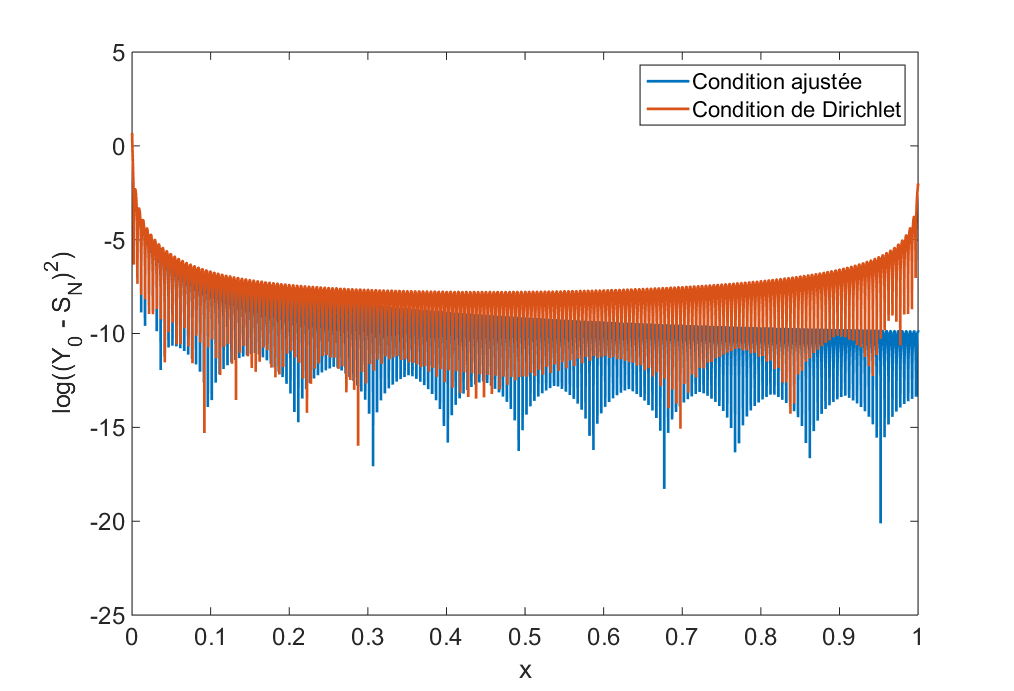
\includegraphics[width=\textwidth]{MeilleureApprox.png} 
\label{MeilleureDecompo}
\caption{Reste du développement en série de Bessel de $x \mapsto Y_0(\mu x)
$ avec conditions de bord ajustée avec $c = -\mu\frac{Y_0'(\mu)}{Y_0(\mu)}$ comme décrit dans le paragraphe précédent (en bleu) et avec une condition de bord non ajustée, condition de Dirichlet ici (en rouge). Dans les deux cas, le développement utilisé pour l'approximation contient les termes $n = 1..200$ et $\mu$ a été fixé à $25$ }
\end{figure}


Les résultats de la partie suivante proposent une explication au fait que ce choix entraîne une meilleure convergence de la série. 

\subsection{Décroissance des coefficients sous conditions}

Nous avons montré dans la section précédente que l'espace $\Lrad$ possède une base Hilbertienne formée des vecteurs propres du Laplacien sur $\D$ avec condition au bord de type
\begin{equation}
\label{condBord}
 \dfrac{\partial f}{\partial r} + c f = 0 \quad \textup{sur }\partial\D
\end{equation}
Nous nous intéressons dans cette section à la décomposition des éléments de $\Lrad$ sur cette base et au comportement des coefficients.
\textbf{Il faut vérifier le travail sur les équivalents de la section précédente généralisé aux conditions de bord de Robin pour vérifier les résultats de cette section}.

\begin{Def} Soit $f\in \Lrad$, on note $c_n(f)$ le coefficient de Fourier généralisé de $f$ dans la base $(e_n)_{n\in\N}$, c'est-à-dire 
\[c_n(f) = \int_\D f(x)e_n(x)dx = c_N \int_{0}^1 r^{N-1} f(rw) e_n(rw) dr \]
Où $w$ est un vecteur unitaire quelconque. 
On appelle développement en série de Bessel l'expression \[ f = \sum_{n=0}^{+\infty} c_n(f) e_n \]

\end{Def}

\begin{Prop} Si $f \in H^2_{rad}(\D) = \enstq{f\in \Hrad}{\forall i \in [1,N], \partial_if \in H^1(\D)}$, on a l'identité 
\[ c_k(f) = -\frac{1}{\lambda_k} c_k(\Delta f) + c_N\left( \dfrac{\partial f}{\partial r}(1) e_n(1) - f(1) \dfrac{\partial e_n}{\partial r}(1)\right)\]
\begin{proof}
Intégration par parties, il faut vérifier les histoires de régularité au bord (thm de traces etc...) 
\end{proof}
\end{Prop}

\begin{Prop} Soit $\Delta^m$ l'opérateur Laplacien itéré $m$ fois et soit $f \in \Lrad$ telle que $\forall i \leq m-1$, $\Delta^i f \in \Lrad$ et vérifie la condition de bord (\ref{condBord}) 
\begin{itemize}
\item[-] Si $\Delta^m f \in \Lrad$ alors on a : 
\begin{equation}
c_k(f) = \dfrac{(-1)^m}{\lambda_k^m}c_k(\Delta^m f)
\label{coeffPair}
 \end{equation}
\item[-] Si $\Delta^m f \in \Hrad$ alors on a : 
\begin{equation}
\label{coeffImpair}
c_k(f) = \dfrac{(-1)^m}{\lambda_k^{m}}\left(\int_{\D}\nabla(\Delta^m f)\cdot\nabla e_n- \int_{\partial\D} \Delta^m f\dfrac{\partial e_n}{\partial r}\right)
\end{equation} 
\end{itemize} 
\begin{proof}
Par récurrence et en utilisant des intégrations par parties.
\end{proof}
\end{Prop}

\begin{Prop} Si $f \in H^m_{rad}$ (c'est-à-dire que les dérivées partielles de $f$ jusqu'à l'ordre $m$ sont dans $L^2$ et $f$ est radiale), et si $\forall i \leq m/2-1$ entier, $\Delta^i f$ vérifie la condition de bord (\ref{condBord}) alors : \[ c_k(f) = O\left(\frac{1}{k^m}\right)\] 
\begin{proof}
On se propose de montrer que $c_k(f) = O\left(\frac{1}{\lambda_k^{m/2}}\right)$ en utilisant la proposition précédente. On disjoint les cas entre $m$ pair et $m$ impair. Si $m$ est pair, c'est facile (remarquer simplement que $c_k(g) \leq \norm{g}_{L^2}$). Si $m$ est impair, il faut contrôler les deux termes entre parenthèses dans la formule (\ref{coeffImpair}). Il est facile de montrer que le premier est contrôlé par $\frac{1}{\sqrt{\lambda_n}}\norm{\nabla(\Delta^m f)}_{L^2}$. Pour le second, la proposition \ref{ExpressionVecteursPropres} de la section précédente permet de borner la valeur de $\frac{\partial e_n}{\partial r}$ sur le bord de $\D$ par $C \sqrt{\lambda_n}$ pour une certaine constante $C$. Enfin, en utilisant les inégalités présentées par exemple dans \cite{de2014elementary} on voit que la valeur de $\Delta^m f$ sur le bord de $\D$ est contrôlée par $\norm{\nabla(\Delta^m f)}_{L^2}$. 
Pour conclure, on utilise $\lambda_k \sim \pi^2k^2$
\end{proof}
\end{Prop}

\begin{Rem} On peut voir que si $f$ est de classe $\mathcal{C}^{2m}$, on a $|c_k(f)| \leq A_N \dfrac{\norm{f^{(2m)}}_{\infty}}{\lambda_k^m}$ où la constante $A_N$ ne dépend que de la dimension $N$. 
\end{Rem}

\begin{Prop} Si $f \in H_{rad}^m$ avec $m > \frac{N+1}{2}$ et si $\forall i \leq m/2-1$ entier, $\Delta^i f$ vérifie la condition de bord (\ref{condBord})  alors la série de Bessel de $f$ converge normalement et on a $\forall x \in \D$ : \[ f(x) = \sum_{k\in \mathbb{N}} c_k(f)e_k(x)\]
\begin{proof}
Utiliser les estimations de la norme $\infty$ des $e_k$ et des coefficients de Fourier de $f$ venant des propositions précédentes pour montrer la convergence normale. 
\end{proof}

\end{Prop}

\subsection{Décomposition sur un anneau intérieur}

Nous sommes intéressés en pratique par l'approximation de fonctions radiales comme combinaisons linéaires finies des vecteurs $e_n$ en utilisant le moins de coefficients possible. Pour un $\varepsilon$ fixé, nous souhaitons trouver le plus petit entier $P$ tel que l'erreur entre $f$ et sa meilleure approximation dans $\Lrad$ par une somme de type $\sum_{p=1}^P\alpha_p e_{n_p}$ soit inférieure à $\varepsilon$. 

La solution à ce problème est de choisir les $P$ plus grands coefficients (en amplitude) de la série de Bessel de $f$, étant donné le caractère orthonormé de la base $(e_n)_{n\in\N}$. Le nombre de $P$ de coefficients dans la décomposition est conditionné par la rapidité de la décroissance des coefficients $c_k(f)$. 

Or, les conditions d'applicabilité des résultats du paragraphe précédent sont restrictives, car la régularité de $f\in \Lrad$ n'est pas une condition suffisante pour assurer la décroissance rapide des coefficients $c_k(f)$. En l'absence de convergence normale, les sommes partielles du développement en série de Bessel présentent un phénomène de type Gibbs, comme l'étudie par exemple \cite{gray1992computer}. 
Dans cette sous-section, nous relâchons l'exigence sur l'erreur en ne demandant une bonne approximation que sur un sous-anneau de $\D$. Nous montrons qu'alors, les coefficients présentent de meilleures propriétés de décroissance rapide. 

\begin{Rem} Le fait de limiter le problème d'approximation sur un sous-anneau permet d'écarter deux difficultés pratiques pour l'approximation des noyaux de Green : 
\begin{itemize}
\item[-] Au voisinage de 0, on écarte le problème les singularités. 
\item[-] Au voisinage de la sphère unité, on va montrer que les conditions de bord sur les dérivées de la fonction à approximer disparaissent.
\end{itemize}
\end{Rem}

\begin{Def} Soit $0 \leq a < b \leq 1$, on note $\mathcal{A}(a,b)$ l'anneau $\enstq{x\in \D}{a \leq |x| \leq b}$. On définit la l'application $\norm{\cdot }_{a,b}$ par $\forall g \in \Lrad $ \[\norm{g}_{a,b} = \sqrt{\int_{\mathcal{A}(a,b)}|g(x)|^2dx}\]
\end{Def}
Par la suite, nous notons $\tilde{e}_n$ la restriction de $e_n$ à l'anneau $\A$. 

\begin{Prop} La famille $(\tilde{e}_n)_{n\in\N}$ est libre et totale dans $\Lradab$
\begin{proof}\text{ }
\begin{itemize}
\item[-] Pour montrer que c'est une famille libre, on écrit que $\Delta e_n = \lambda_n e_n$ et on utilise un déterminant de Van Der Monde. 
\item[-] Pour montrer qu'elle est totale, il suffit de remarquer que si $f\in \Lradab$, la fonction $g$ de coïncidant avec $f$ sur $\Lradab$ et prolongée par $0$ sur $\D \setminus \A$ est un élément de $\Lrad$. On voit alors que $\norm{f - \sum_{^p=1}^P \duality{f}{e_p}\tilde{e}_p}_{\Lradab} \leq \norm{f - \sum_{^p=1}^P \duality{f}{e_p}e_p}_{\Lrad} \to 0$ lorsque $P \to +\infty$. 
\end{itemize}
\end{proof}
\end{Prop}

\begin{Prop} Il existe une base Hilbertienne $(f_n)_{n \in \mathbb{N}}$ de $\Lradab$ telle que $\forall n \in \N$, \[f_n \in \textup{Vect}\left(\{(\tilde{e}_k)_{k \leq n} \}\right)\]
\begin{proof} Gram-Schmidt.
\end{proof}
\end{Prop}


\begin{Prop} Si $n \neq m$, on a en notant $k = \frac{N}{2}-1$ : \[ \duality{\tilde{e}_n}{\tilde{e}_m}_{\Lradab} =\frac{2} {(\lambda_n - \lambda_m)J_{k+1}(\rho_n)J_{k+1}(\rho_m)}\left[ \rho_m r J_k(\rho_n r)J_k'(\rho_m r)- \rho_n r J_k'(\rho_n r )J_k(\rho_m r)\right]^b_a\] 
et \[ \norm{\tilde{e}_n}^2_{\Lradab} =  \frac{2} {J_{k+1}(\rho_n)^2}\left[ \frac{r^2}{2}\left(J_k(\rho_n r)^2 + J_{k}'(\rho_n r)^2\right)\right]_a^b\]
où la notation $[f]_a^b$ est utilisée pour $f(b) - f(a)$.
\begin{proof}
La flemme pour le moment. L'idée est d'utiliser deux IPP successives. 
\end{proof}
\end{Prop}

\begin{Rem} L'évaluation du produit scalaire ne demande pas d'évaluer d'intégrale, ce qui est avantageux lors de l'implantation de l'orthonormalisation de Gram-Schmidt. 
\end{Rem}



\bibliographystyle{plain}
\bibliography{biblio} 

\end{document}
